\documentclass[1p]{elsarticle_modified}
%\bibliographystyle{elsarticle-num}

%\usepackage[colorlinks]{hyperref}
%\usepackage{abbrmath_seonhwa} %\Abb, \Ascr, \Acal ,\Abf, \Afrak
\usepackage{amsfonts}
\usepackage{amssymb}
\usepackage{amsmath}
\usepackage{amsthm}
\usepackage{scalefnt}
\usepackage{amsbsy}
\usepackage{kotex}
\usepackage{caption}
\usepackage{subfig}
\usepackage{color}
\usepackage{graphicx}
\usepackage{xcolor} %% white, black, red, green, blue, cyan, magenta, yellow
\usepackage{float}
\usepackage{setspace}
\usepackage{hyperref}

\usepackage{tikz}
\usetikzlibrary{arrows}

\usepackage{multirow}
\usepackage{array} % fixed length table
\usepackage{hhline}

%%%%%%%%%%%%%%%%%%%%%
\makeatletter
\renewcommand*\env@matrix[1][\arraystretch]{%
	\edef\arraystretch{#1}%
	\hskip -\arraycolsep
	\let\@ifnextchar\new@ifnextchar
	\array{*\c@MaxMatrixCols c}}
\makeatother %https://tex.stackexchange.com/questions/14071/how-can-i-increase-the-line-spacing-in-a-matrix
%%%%%%%%%%%%%%%

\usepackage[normalem]{ulem}

\newcommand{\msout}[1]{\ifmmode\text{\sout{\ensuremath{#1}}}\else\sout{#1}\fi}
%SOURCE: \msout is \stkout macro in https://tex.stackexchange.com/questions/20609/strikeout-in-math-mode

\newcommand{\cancel}[1]{
	\ifmmode
	{\color{red}\msout{#1}}
	\else
	{\color{red}\sout{#1}}
	\fi
}

\newcommand{\add}[1]{
	{\color{blue}\uwave{#1}}
}

\newcommand{\replace}[2]{
	\ifmmode
	{\color{red}\msout{#1}}{\color{blue}\uwave{#2}}
	\else
	{\color{red}\sout{#1}}{\color{blue}\uwave{#2}}
	\fi
}

\newcommand{\Sol}{\mathcal{S}} %segment
\newcommand{\D}{D} %diagram
\newcommand{\A}{\mathcal{A}} %arc


%%%%%%%%%%%%%%%%%%%%%%%%%%%%%5 test

\def\sl{\operatorname{\textup{SL}}(2,\Cbb)}
\def\psl{\operatorname{\textup{PSL}}(2,\Cbb)}
\def\quan{\mkern 1mu \triangleright \mkern 1mu}

\theoremstyle{definition}
\newtheorem{thm}{Theorem}[section]
\newtheorem{prop}[thm]{Proposition}
\newtheorem{lem}[thm]{Lemma}
\newtheorem{ques}[thm]{Question}
\newtheorem{cor}[thm]{Corollary}
\newtheorem{defn}[thm]{Definition}
\newtheorem{exam}[thm]{Example}
\newtheorem{rmk}[thm]{Remark}
\newtheorem{alg}[thm]{Algorithm}

\newcommand{\I}{\sqrt{-1}}
\begin{document}

%\begin{frontmatter}
%
%\title{Boundary parabolic representations of knots up to 8 crossings}
%
%%% Group authors per affiliation:
%\author{Yunhi Cho} 
%\address{Department of Mathematics, University of Seoul, Seoul, Korea}
%\ead{yhcho@uos.ac.kr}
%
%
%\author{Seonhwa Kim} %\fnref{s_kim}}
%\address{Center for Geometry and Physics, Institute for Basic Science, Pohang, 37673, Korea}
%\ead{ryeona17@ibs.re.kr}
%
%\author{Hyuk Kim}
%\address{Department of Mathematical Sciences, Seoul National University, Seoul 08826, Korea}
%\ead{hyukkim@snu.ac.kr}
%
%\author{Seokbeom Yoon}
%\address{Department of Mathematical Sciences, Seoul National University, Seoul, 08826,  Korea}
%\ead{sbyoon15@snu.ac.kr}
%
%\begin{abstract}
%We find all boundary parabolic representation of knots up to 8 crossings.
%
%\end{abstract}
%\begin{keyword}
%    \MSC[2010] 57M25 
%\end{keyword}
%
%\end{frontmatter}

%\linenumbers
%\tableofcontents
%
\newcommand\colored[1]{\textcolor{white}{\rule[-0.35ex]{0.8em}{1.4ex}}\kern-0.8em\color{red} #1}%
%\newcommand\colored[1]{\textcolor{white}{ #1}\kern-2.17ex	\textcolor{white}{ #1}\kern-1.81ex	\textcolor{white}{ #1}\kern-2.15ex\color{red}#1	}

{\Large $\underline{12n_{0285}~(K12n_{0285})}$}

\setlength{\tabcolsep}{10pt}
\renewcommand{\arraystretch}{1.6}
\vspace{1cm}\begin{tabular}{m{100pt}>{\centering\arraybackslash}m{274pt}}
\multirow{5}{120pt}{
	\centering
	\includegraphics[width=112pt]{../../../GIT/diagram.site/Diagrams/png/2374_12n_0285.png}\\
\ \ \ A knot diagram\footnotemark}&
\allowdisplaybreaks
\textbf{Linearized knot diagam} \\
\cline{2-2}
 &
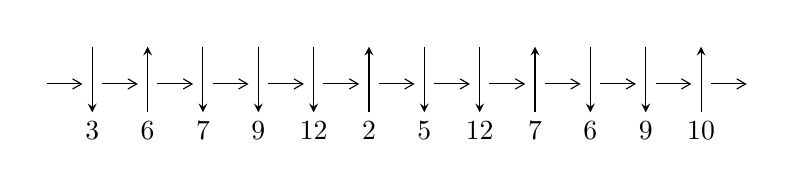
\begin{tikzpicture}[x=20pt, y=17pt]
	% nodes
	\node (C0) at (0, 0) {};
	\node (C1) at (1, 0) {};
	\node (C1U) at (1, +1) {};
	\node (C1D) at (1, -1) {3};

	\node (C2) at (2, 0) {};
	\node (C2U) at (2, +1) {};
	\node (C2D) at (2, -1) {6};

	\node (C3) at (3, 0) {};
	\node (C3U) at (3, +1) {};
	\node (C3D) at (3, -1) {7};

	\node (C4) at (4, 0) {};
	\node (C4U) at (4, +1) {};
	\node (C4D) at (4, -1) {9};

	\node (C5) at (5, 0) {};
	\node (C5U) at (5, +1) {};
	\node (C5D) at (5, -1) {12};

	\node (C6) at (6, 0) {};
	\node (C6U) at (6, +1) {};
	\node (C6D) at (6, -1) {2};

	\node (C7) at (7, 0) {};
	\node (C7U) at (7, +1) {};
	\node (C7D) at (7, -1) {5};

	\node (C8) at (8, 0) {};
	\node (C8U) at (8, +1) {};
	\node (C8D) at (8, -1) {12};

	\node (C9) at (9, 0) {};
	\node (C9U) at (9, +1) {};
	\node (C9D) at (9, -1) {7};

	\node (C10) at (10, 0) {};
	\node (C10U) at (10, +1) {};
	\node (C10D) at (10, -1) {6};

	\node (C11) at (11, 0) {};
	\node (C11U) at (11, +1) {};
	\node (C11D) at (11, -1) {9};

	\node (C12) at (12, 0) {};
	\node (C12U) at (12, +1) {};
	\node (C12D) at (12, -1) {10};
	\node (C13) at (13, 0) {};

	% arrows
	\draw[->,>={angle 60}]
	(C0) edge (C1) (C1) edge (C2) (C2) edge (C3) (C3) edge (C4) (C4) edge (C5) (C5) edge (C6) (C6) edge (C7) (C7) edge (C8) (C8) edge (C9) (C9) edge (C10) (C10) edge (C11) (C11) edge (C12) (C12) edge (C13) ;	\draw[->,>=stealth]
	(C1U) edge (C1D) (C2D) edge (C2U) (C3U) edge (C3D) (C4U) edge (C4D) (C5U) edge (C5D) (C6D) edge (C6U) (C7U) edge (C7D) (C8U) edge (C8D) (C9D) edge (C9U) (C10U) edge (C10D) (C11U) edge (C11D) (C12D) edge (C12U) ;
	\end{tikzpicture} \\
\hhline{~~} \\& 
\textbf{Solving Sequence} \\ \cline{2-2} 
 &
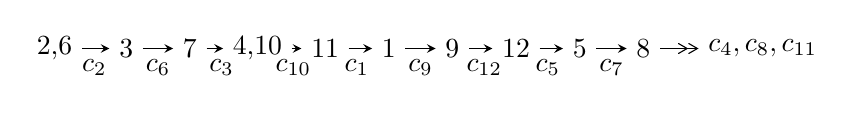
\begin{tikzpicture}[x=23pt, y=7pt]
	% node
	\node (A0) at (-1/8, 0) {2,6};
	\node (A1) at (1, 0) {3};
	\node (A2) at (2, 0) {7};
	\node (A3) at (49/16, 0) {4,10};
	\node (A4) at (33/8, 0) {11};
	\node (A5) at (41/8, 0) {1};
	\node (A6) at (49/8, 0) {9};
	\node (A7) at (57/8, 0) {12};
	\node (A8) at (65/8, 0) {5};
	\node (A9) at (73/8, 0) {8};
	\node (C1) at (1/2, -1) {$c_{2}$};
	\node (C2) at (3/2, -1) {$c_{6}$};
	\node (C3) at (5/2, -1) {$c_{3}$};
	\node (C4) at (29/8, -1) {$c_{10}$};
	\node (C5) at (37/8, -1) {$c_{1}$};
	\node (C6) at (45/8, -1) {$c_{9}$};
	\node (C7) at (53/8, -1) {$c_{12}$};
	\node (C8) at (61/8, -1) {$c_{5}$};
	\node (C9) at (69/8, -1) {$c_{7}$};
	\node (A10) at (11, 0) {$c_{4},c_{8},c_{11}$};

	% edge
	\draw[->,>=stealth]	
	(A0) edge (A1) (A1) edge (A2) (A2) edge (A3) (A3) edge (A4) (A4) edge (A5) (A5) edge (A6) (A6) edge (A7) (A7) edge (A8) (A8) edge (A9) ;
	\draw[->>,>={angle 60}]	
	(A9) edge (A10);
\end{tikzpicture} \\ 

\end{tabular} \\

\footnotetext{
The image of knot diagram is generated by the software ``\textbf{Draw programme}" developed by Andrew Bartholomew(\url{http://www.layer8.co.uk/maths/draw/index.htm\#Running-draw}), where we modified some parts for our purpose(\url{https://github.com/CATsTAILs/LinksPainter}).
}\phantom \\ \newline 
\centering \textbf{Ideals for irreducible components\footnotemark of $X_{\text{par}}$} 
 
\begin{align*}
I^u_{1}&=\langle 
u^{16}+4 u^{15}+\cdots+b-1,\;- u^{16}-3 u^{15}+\cdots+2 a-3,\;u^{17}+5 u^{16}+\cdots-3 u-2\rangle \\
I^u_{2}&=\langle 
- u^9+2 u^8-4 u^7+4 u^6-6 u^5+4 u^4-5 u^3+2 u^2+b-2 u+1,\\
\phantom{I^u_{2}}&\phantom{= \langle  }-2 u^9+3 u^8-6 u^7+4 u^6-8 u^5+4 u^4-7 u^3+u^2+a-3 u+2,\\
\phantom{I^u_{2}}&\phantom{= \langle  }u^{10}-2 u^9+4 u^8-4 u^7+6 u^6-5 u^5+6 u^4-3 u^3+3 u^2-2 u+1\rangle \\
I^u_{3}&=\langle 
- u^5+u^4+u^2 a- a u- u^2+b- u+1,\;u^5 a+2 u^5+u^4- u^3+a^2+3 a u+u^2+4 u+4,\\
\phantom{I^u_{3}}&\phantom{= \langle  }u^6- u^5+u^4+2 u^2- u+1\rangle \\
\\
\end{align*}
\raggedright * 3 irreducible components of $\dim_{\mathbb{C}}=0$, with total 39 representations.\\
\footnotetext{All coefficients of polynomials are rational numbers. But the coefficients are sometimes approximated in decimal forms when there is not enough margin.}
\newpage
\renewcommand{\arraystretch}{1}
\centering \section*{I. $I^u_{1}= \langle u^{16}+4 u^{15}+\cdots+b-1,\;- u^{16}-3 u^{15}+\cdots+2 a-3,\;u^{17}+5 u^{16}+\cdots-3 u-2 \rangle$}
\flushleft \textbf{(i) Arc colorings}\\
\begin{tabular}{m{7pt} m{180pt} m{7pt} m{180pt} }
\flushright $a_{2}=$&$\begin{pmatrix}1\\0\end{pmatrix}$ \\
\flushright $a_{6}=$&$\begin{pmatrix}0\\u\end{pmatrix}$ \\
\flushright $a_{3}=$&$\begin{pmatrix}1\\- u^2\end{pmatrix}$ \\
\flushright $a_{7}=$&$\begin{pmatrix}u\\u\end{pmatrix}$ \\
\flushright $a_{4}=$&$\begin{pmatrix}u^4+u^2+1\\u^4\end{pmatrix}$ \\
\flushright $a_{10}=$&$\begin{pmatrix}\frac{1}{2} u^{16}+\frac{3}{2} u^{15}+\cdots-\frac{1}{2} u+\frac{3}{2}\\- u^{16}-4 u^{15}+\cdots- u+1\end{pmatrix}$ \\
\flushright $a_{11}=$&$\begin{pmatrix}\frac{1}{2} u^{16}+\frac{3}{2} u^{15}+\cdots-\frac{1}{2} u+\frac{3}{2}\\u^{16}+3 u^{15}+\cdots-3 u-1\end{pmatrix}$ \\
\flushright $a_{1}=$&$\begin{pmatrix}u^2+1\\- u^4\end{pmatrix}$ \\
\flushright $a_{9}=$&$\begin{pmatrix}\frac{3}{2} u^{16}+\frac{15}{2} u^{15}+\cdots-\frac{7}{2} u-\frac{5}{2}\\2 u^{15}+7 u^{14}+\cdots-4 u-3\end{pmatrix}$ \\
\flushright $a_{12}=$&$\begin{pmatrix}\frac{3}{2} u^{16}+\frac{15}{2} u^{15}+\cdots-\frac{7}{2} u-\frac{5}{2}\\2 u^{16}+9 u^{15}+\cdots-4 u-3\end{pmatrix}$ \\
\flushright $a_{5}=$&$\begin{pmatrix}\frac{1}{2} u^{16}+\frac{3}{2} u^{15}+\cdots-\frac{1}{2} u+\frac{1}{2}\\- u^{16}-6 u^{15}+\cdots+3 u+3\end{pmatrix}$ \\
\flushright $a_{8}=$&$\begin{pmatrix}-\frac{5}{2} u^{16}-\frac{27}{2} u^{15}+\cdots+\frac{13}{2} u+\frac{13}{2}\\-2 u^{16}-12 u^{15}+\cdots+6 u+7\end{pmatrix}$\\&\end{tabular}
\flushleft \textbf{(ii) Obstruction class $= -1$}\\~\\
\flushleft \textbf{(iii) Cusp Shapes $= - u^{16}-6 u^{15}-20 u^{14}-43 u^{13}-71 u^{12}-91 u^{11}-94 u^{10}-58 u^9+66 u^7+87 u^6+92 u^5+60 u^4+46 u^3+17 u^2+17 u-4$}\\~\\
\newpage\renewcommand{\arraystretch}{1}
\flushleft \textbf{(iv) u-Polynomials at the component}\newline \\
\begin{tabular}{m{50pt}|m{274pt}}
Crossings & \hspace{64pt}u-Polynomials at each crossing \\
\hline $$\begin{aligned}c_{1}\end{aligned}$$&$\begin{aligned}
&u^{17}+5 u^{16}+\cdots-35 u-4
\end{aligned}$\\
\hline $$\begin{aligned}c_{2},c_{6}\end{aligned}$$&$\begin{aligned}
&u^{17}-5 u^{16}+\cdots-3 u+2
\end{aligned}$\\
\hline $$\begin{aligned}c_{3}\end{aligned}$$&$\begin{aligned}
&u^{17}+5 u^{16}+\cdots+201 u+74
\end{aligned}$\\
\hline $$\begin{aligned}c_{4},c_{10}\end{aligned}$$&$\begin{aligned}
&u^{17}+13 u^{15}+\cdots+4 u+1
\end{aligned}$\\
\hline $$\begin{aligned}c_{5},c_{7}\end{aligned}$$&$\begin{aligned}
&u^{17}- u^{16}+\cdots+2 u+1
\end{aligned}$\\
\hline $$\begin{aligned}c_{8},c_{11}\end{aligned}$$&$\begin{aligned}
&u^{17}-10 u^{16}+\cdots+27 u-4
\end{aligned}$\\
\hline $$\begin{aligned}c_{9},c_{12}\end{aligned}$$&$\begin{aligned}
&u^{17}+3 u^{16}+\cdots-8 u+1
\end{aligned}$\\
\hline
\end{tabular}\\~\\
\newpage\renewcommand{\arraystretch}{1}
\flushleft \textbf{(v) Riley Polynomials at the component}\newline \\
\begin{tabular}{m{50pt}|m{274pt}}
Crossings & \hspace{64pt}Riley Polynomials at each crossing \\
\hline $$\begin{aligned}c_{1}\end{aligned}$$&$\begin{aligned}
&y^{17}+17 y^{16}+\cdots+49 y-16
\end{aligned}$\\
\hline $$\begin{aligned}c_{2},c_{6}\end{aligned}$$&$\begin{aligned}
&y^{17}+5 y^{16}+\cdots-35 y-4
\end{aligned}$\\
\hline $$\begin{aligned}c_{3}\end{aligned}$$&$\begin{aligned}
&y^{17}+29 y^{16}+\cdots-126395 y-5476
\end{aligned}$\\
\hline $$\begin{aligned}c_{4},c_{10}\end{aligned}$$&$\begin{aligned}
&y^{17}+26 y^{16}+\cdots-10 y-1
\end{aligned}$\\
\hline $$\begin{aligned}c_{5},c_{7}\end{aligned}$$&$\begin{aligned}
&y^{17}-25 y^{16}+\cdots+4 y-1
\end{aligned}$\\
\hline $$\begin{aligned}c_{8},c_{11}\end{aligned}$$&$\begin{aligned}
&y^{17}+2 y^{16}+\cdots-143 y-16
\end{aligned}$\\
\hline $$\begin{aligned}c_{9},c_{12}\end{aligned}$$&$\begin{aligned}
&y^{17}-15 y^{16}+\cdots+16 y-1
\end{aligned}$\\
\hline
\end{tabular}\\~\\
\newpage\flushleft \textbf{(vi) Complex Volumes and Cusp Shapes}
$$\begin{array}{c|c|c}  
\text{Solutions to }I^u_{1}& \I (\text{vol} + \sqrt{-1}CS) & \text{Cusp shape}\\
 \hline 
\begin{aligned}
u &= \phantom{-}0.999402\phantom{ +0.000000I} \\
a &= \phantom{-}0.387652\phantom{ +0.000000I} \\
b &= -0.774608\phantom{ +0.000000I}\end{aligned}
 & -3.45333\phantom{ +0.000000I} & -1.57930\phantom{ +0.000000I} \\ \hline\begin{aligned}
u &= -0.225183 + 0.839513 I \\
a &= \phantom{-}0.457066 - 0.305622 I \\
b &= \phantom{-}0.260858 - 0.479622 I\end{aligned}
 & -0.515123 - 1.230730 I & -4.57965 + 6.11157 I \\ \hline\begin{aligned}
u &= -0.225183 - 0.839513 I \\
a &= \phantom{-}0.457066 + 0.305622 I \\
b &= \phantom{-}0.260858 + 0.479622 I\end{aligned}
 & -0.515123 + 1.230730 I & -4.57965 - 6.11157 I \\ \hline\begin{aligned}
u &= -0.902975 + 0.779498 I \\
a &= -0.37268 + 1.47715 I \\
b &= -1.18710 + 0.79283 I\end{aligned}
 & \phantom{-}5.52032 - 2.59660 I & -1.98291 + 2.57071 I \\ \hline\begin{aligned}
u &= -0.902975 - 0.779498 I \\
a &= -0.37268 - 1.47715 I \\
b &= -1.18710 - 0.79283 I\end{aligned}
 & \phantom{-}5.52032 + 2.59660 I & -1.98291 - 2.57071 I \\ \hline\begin{aligned}
u &= -1.013990 + 0.825716 I \\
a &= \phantom{-}1.04491 - 1.15054 I \\
b &= \phantom{-}1.67420 + 0.11880 I\end{aligned}
 & \phantom{-}2.66130 + 5.14311 I & -3.31224 - 2.06906 I \\ \hline\begin{aligned}
u &= -1.013990 - 0.825716 I \\
a &= \phantom{-}1.04491 + 1.15054 I \\
b &= \phantom{-}1.67420 - 0.11880 I\end{aligned}
 & \phantom{-}2.66130 - 5.14311 I & -3.31224 + 2.06906 I \\ \hline\begin{aligned}
u &= -0.792289 + 1.041050 I \\
a &= -1.139370 + 0.603283 I \\
b &= -1.78949 + 0.05972 I\end{aligned}
 & \phantom{-}4.68149 - 3.71646 I & -2.79518 + 2.82261 I \\ \hline\begin{aligned}
u &= -0.792289 - 1.041050 I \\
a &= -1.139370 - 0.603283 I \\
b &= -1.78949 - 0.05972 I\end{aligned}
 & \phantom{-}4.68149 + 3.71646 I & -2.79518 - 2.82261 I \\ \hline\begin{aligned}
u &= \phantom{-}0.065367 + 0.651578 I \\
a &= \phantom{-}0.870762 - 0.440011 I \\
b &= -0.015136 - 0.797710 I\end{aligned}
 & -0.691744 - 1.119700 I & -6.04337 + 5.63794 I\\
 \hline 
 \end{array}$$\newpage$$\begin{array}{c|c|c}  
\text{Solutions to }I^u_{1}& \I (\text{vol} + \sqrt{-1}CS) & \text{Cusp shape}\\
 \hline 
\begin{aligned}
u &= \phantom{-}0.065367 - 0.651578 I \\
a &= \phantom{-}0.870762 + 0.440011 I \\
b &= -0.015136 + 0.797710 I\end{aligned}
 & -0.691744 + 1.119700 I & -6.04337 - 5.63794 I \\ \hline\begin{aligned}
u &= \phantom{-}0.354914 + 0.549103 I \\
a &= -0.916291 + 0.819903 I \\
b &= \phantom{-}0.934133 + 0.713219 I\end{aligned}
 & \phantom{-}0.02980 + 3.01264 I & -7.09672 + 0.35044 I \\ \hline\begin{aligned}
u &= \phantom{-}0.354914 - 0.549103 I \\
a &= -0.916291 - 0.819903 I \\
b &= \phantom{-}0.934133 - 0.713219 I\end{aligned}
 & \phantom{-}0.02980 - 3.01264 I & -7.09672 - 0.35044 I \\ \hline\begin{aligned}
u &= \phantom{-}0.398162 + 1.288650 I \\
a &= -0.300696 - 0.167666 I \\
b &= -0.720067 + 0.510972 I\end{aligned}
 & -7.74200 + 4.95608 I & -4.59429 - 5.14858 I \\ \hline\begin{aligned}
u &= \phantom{-}0.398162 - 1.288650 I \\
a &= -0.300696 + 0.167666 I \\
b &= -0.720067 - 0.510972 I\end{aligned}
 & -7.74200 - 4.95608 I & -4.59429 + 5.14858 I \\ \hline\begin{aligned}
u &= -0.883711 + 1.061310 I \\
a &= \phantom{-}0.91247 - 1.36079 I \\
b &= \phantom{-}2.22990 - 0.92943 I\end{aligned}
 & \phantom{-}1.89495 - 12.06910 I & -4.30600 + 6.19242 I \\ \hline\begin{aligned}
u &= -0.883711 - 1.061310 I \\
a &= \phantom{-}0.91247 + 1.36079 I \\
b &= \phantom{-}2.22990 + 0.92943 I\end{aligned}
 & \phantom{-}1.89495 + 12.06910 I & -4.30600 - 6.19242 I\\
 \hline 
 \end{array}$$\newpage\newpage\renewcommand{\arraystretch}{1}
\centering \section*{II. $I^u_{2}= \langle - u^9+2 u^8+\cdots+b+1,\;-2 u^9+3 u^8+\cdots+a+2,\;u^{10}-2 u^9+\cdots-2 u+1 \rangle$}
\flushleft \textbf{(i) Arc colorings}\\
\begin{tabular}{m{7pt} m{180pt} m{7pt} m{180pt} }
\flushright $a_{2}=$&$\begin{pmatrix}1\\0\end{pmatrix}$ \\
\flushright $a_{6}=$&$\begin{pmatrix}0\\u\end{pmatrix}$ \\
\flushright $a_{3}=$&$\begin{pmatrix}1\\- u^2\end{pmatrix}$ \\
\flushright $a_{7}=$&$\begin{pmatrix}u\\u\end{pmatrix}$ \\
\flushright $a_{4}=$&$\begin{pmatrix}u^4+u^2+1\\u^4\end{pmatrix}$ \\
\flushright $a_{10}=$&$\begin{pmatrix}2 u^9-3 u^8+6 u^7-4 u^6+8 u^5-4 u^4+7 u^3- u^2+3 u-2\\u^9-2 u^8+4 u^7-4 u^6+6 u^5-4 u^4+5 u^3-2 u^2+2 u-1\end{pmatrix}$ \\
\flushright $a_{11}=$&$\begin{pmatrix}2 u^9-3 u^8+6 u^7-4 u^6+8 u^5-4 u^4+7 u^3- u^2+3 u-2\\u^9-2 u^8+4 u^7-4 u^6+6 u^5-5 u^4+5 u^3-3 u^2+2 u-2\end{pmatrix}$ \\
\flushright $a_{1}=$&$\begin{pmatrix}u^2+1\\- u^4\end{pmatrix}$ \\
\flushright $a_{9}=$&$\begin{pmatrix}2 u^9-3 u^8+6 u^7-5 u^6+9 u^5-6 u^4+8 u^3-3 u^2+4 u-3\\u^9-2 u^8+4 u^7-5 u^6+7 u^5-6 u^4+6 u^3-4 u^2+3 u-2\end{pmatrix}$ \\
\flushright $a_{12}=$&$\begin{pmatrix}-2 u^9+3 u^8-6 u^7+5 u^6-9 u^5+6 u^4-8 u^3+3 u^2-4 u+3\\- u^9+u^8-2 u^7+u^6-3 u^5+u^4-3 u^3+u^2-2 u+1\end{pmatrix}$ \\
\flushright $a_{5}=$&$\begin{pmatrix}-3 u^9+5 u^8-10 u^7+8 u^6-14 u^5+10 u^4-13 u^3+4 u^2-6 u+5\\- u^9+2 u^8-4 u^7+3 u^6-5 u^5+4 u^4-5 u^3+u^2-2 u+2\end{pmatrix}$ \\
\flushright $a_{8}=$&$\begin{pmatrix}6 u^9-9 u^8+18 u^7-14 u^6+26 u^5-16 u^4+23 u^3-7 u^2+11 u-8\\3 u^9-4 u^8+8 u^7-6 u^6+12 u^5-6 u^4+10 u^3-3 u^2+5 u-3\end{pmatrix}$\\&\end{tabular}
\flushleft \textbf{(ii) Obstruction class $= 1$}\\~\\
\flushleft \textbf{(iii) Cusp Shapes $= - u^9+4 u^8-5 u^7+5 u^6-2 u^5+u^4+3 u^3-4 u^2+5 u-6$}\\~\\
\newpage\renewcommand{\arraystretch}{1}
\flushleft \textbf{(iv) u-Polynomials at the component}\newline \\
\begin{tabular}{m{50pt}|m{274pt}}
Crossings & \hspace{64pt}u-Polynomials at each crossing \\
\hline $$\begin{aligned}c_{1}\end{aligned}$$&$\begin{aligned}
&u^{10}-4 u^9+12 u^8-24 u^7+38 u^6-41 u^5+34 u^4-19 u^3+9 u^2-2 u+1
\end{aligned}$\\
\hline $$\begin{aligned}c_{2}\end{aligned}$$&$\begin{aligned}
&u^{10}-2 u^9+4 u^8-4 u^7+6 u^6-5 u^5+6 u^4-3 u^3+3 u^2-2 u+1
\end{aligned}$\\
\hline $$\begin{aligned}c_{3}\end{aligned}$$&$\begin{aligned}
&u^{10}+2 u^9+8 u^8+4 u^7+10 u^5+u^4-6 u^3+16 u^2-10 u+5
\end{aligned}$\\
\hline $$\begin{aligned}c_{4},c_{10}\end{aligned}$$&$\begin{aligned}
&u^{10}+u^8+4 u^7-11 u^6-5 u^5+18 u^4-6 u^3-2 u+1
\end{aligned}$\\
\hline $$\begin{aligned}c_{5},c_{7}\end{aligned}$$&$\begin{aligned}
&u^{10}+u^9-4 u^8-5 u^7-3 u^6+u^5+15 u^4+15 u^3+11 u^2+4 u+1
\end{aligned}$\\
\hline $$\begin{aligned}c_{6}\end{aligned}$$&$\begin{aligned}
&u^{10}+2 u^9+4 u^8+4 u^7+6 u^6+5 u^5+6 u^4+3 u^3+3 u^2+2 u+1
\end{aligned}$\\
\hline $$\begin{aligned}c_{8}\end{aligned}$$&$\begin{aligned}
&u^{10}-7 u^9+19 u^8-24 u^7+9 u^6+16 u^5-27 u^4+13 u^3+6 u^2-10 u+5
\end{aligned}$\\
\hline $$\begin{aligned}c_{9},c_{12}\end{aligned}$$&$\begin{aligned}
&u^{10}-3 u^9+u^8+4 u^7-5 u^6+6 u^4- u^3- u^2+2 u+1
\end{aligned}$\\
\hline $$\begin{aligned}c_{11}\end{aligned}$$&$\begin{aligned}
&u^{10}+7 u^9+19 u^8+24 u^7+9 u^6-16 u^5-27 u^4-13 u^3+6 u^2+10 u+5
\end{aligned}$\\
\hline
\end{tabular}\\~\\
\newpage\renewcommand{\arraystretch}{1}
\flushleft \textbf{(v) Riley Polynomials at the component}\newline \\
\begin{tabular}{m{50pt}|m{274pt}}
Crossings & \hspace{64pt}Riley Polynomials at each crossing \\
\hline $$\begin{aligned}c_{1}\end{aligned}$$&$\begin{aligned}
&y^{10}+8 y^9+\cdots+14 y+1
\end{aligned}$\\
\hline $$\begin{aligned}c_{2},c_{6}\end{aligned}$$&$\begin{aligned}
&y^{10}+4 y^9+12 y^8+24 y^7+38 y^6+41 y^5+34 y^4+19 y^3+9 y^2+2 y+1
\end{aligned}$\\
\hline $$\begin{aligned}c_{3}\end{aligned}$$&$\begin{aligned}
&y^{10}+12 y^9+\cdots+60 y+25
\end{aligned}$\\
\hline $$\begin{aligned}c_{4},c_{10}\end{aligned}$$&$\begin{aligned}
&y^{10}+2 y^9+\cdots-4 y+1
\end{aligned}$\\
\hline $$\begin{aligned}c_{5},c_{7}\end{aligned}$$&$\begin{aligned}
&y^{10}-9 y^9+\cdots+6 y+1
\end{aligned}$\\
\hline $$\begin{aligned}c_{8},c_{11}\end{aligned}$$&$\begin{aligned}
&y^{10}-11 y^9+\cdots-40 y+25
\end{aligned}$\\
\hline $$\begin{aligned}c_{9},c_{12}\end{aligned}$$&$\begin{aligned}
&y^{10}-7 y^9+\cdots-6 y+1
\end{aligned}$\\
\hline
\end{tabular}\\~\\
\newpage\flushleft \textbf{(vi) Complex Volumes and Cusp Shapes}
$$\begin{array}{c|c|c}  
\text{Solutions to }I^u_{2}& \I (\text{vol} + \sqrt{-1}CS) & \text{Cusp shape}\\
 \hline 
\begin{aligned}
u &= -0.378370 + 0.962478 I \\
a &= \phantom{-}0.467882 + 0.091620 I \\
b &= \phantom{-}0.034500 + 0.828197 I\end{aligned}
 & -0.560424 - 0.074153 I & -4.22332 - 0.05050 I \\ \hline\begin{aligned}
u &= -0.378370 - 0.962478 I \\
a &= \phantom{-}0.467882 - 0.091620 I \\
b &= \phantom{-}0.034500 - 0.828197 I\end{aligned}
 & -0.560424 + 0.074153 I & -4.22332 + 0.05050 I \\ \hline\begin{aligned}
u &= -0.549385 + 0.711068 I \\
a &= -0.483620 - 0.417086 I \\
b &= \phantom{-}0.789580 - 0.577598 I\end{aligned}
 & \phantom{-}0.35639 - 3.68459 I & -1.74176 + 8.84832 I \\ \hline\begin{aligned}
u &= -0.549385 - 0.711068 I \\
a &= -0.483620 + 0.417086 I \\
b &= \phantom{-}0.789580 + 0.577598 I\end{aligned}
 & \phantom{-}0.35639 + 3.68459 I & -1.74176 - 8.84832 I \\ \hline\begin{aligned}
u &= \phantom{-}0.485122 + 1.143680 I \\
a &= \phantom{-}0.522993 - 0.643782 I \\
b &= \phantom{-}0.836616 - 0.985073 I\end{aligned}
 & -8.64742 + 3.94137 I & -8.44290 - 2.10467 I \\ \hline\begin{aligned}
u &= \phantom{-}0.485122 - 1.143680 I \\
a &= \phantom{-}0.522993 + 0.643782 I \\
b &= \phantom{-}0.836616 + 0.985073 I\end{aligned}
 & -8.64742 - 3.94137 I & -8.44290 + 2.10467 I \\ \hline\begin{aligned}
u &= \phantom{-}0.946362 + 0.955964 I \\
a &= -0.97616 - 1.25675 I \\
b &= -2.01415 - 0.37924 I\end{aligned}
 & \phantom{-}10.15450 + 3.46808 I & \phantom{-}1.22554 - 2.41931 I \\ \hline\begin{aligned}
u &= \phantom{-}0.946362 - 0.955964 I \\
a &= -0.97616 + 1.25675 I \\
b &= -2.01415 + 0.37924 I\end{aligned}
 & \phantom{-}10.15450 - 3.46808 I & \phantom{-}1.22554 + 2.41931 I \\ \hline\begin{aligned}
u &= \phantom{-}0.496271 + 0.410325 I \\
a &= -1.53110 + 1.96143 I \\
b &= -0.646542 + 0.815887 I\end{aligned}
 & -6.23787 + 0.27295 I & -4.31756 + 1.10366 I \\ \hline\begin{aligned}
u &= \phantom{-}0.496271 - 0.410325 I \\
a &= -1.53110 - 1.96143 I \\
b &= -0.646542 - 0.815887 I\end{aligned}
 & -6.23787 - 0.27295 I & -4.31756 - 1.10366 I\\
 \hline 
 \end{array}$$\newpage\newpage\renewcommand{\arraystretch}{1}
\centering \section*{III. $I^u_{3}= \langle - u^5+u^4+u^2 a- a u- u^2+b- u+1,\;u^5 a+2 u^5+u^4- u^3+a^2+3 a u+u^2+4 u+4,\;u^6- u^5+u^4+2 u^2- u+1 \rangle$}
\flushleft \textbf{(i) Arc colorings}\\
\begin{tabular}{m{7pt} m{180pt} m{7pt} m{180pt} }
\flushright $a_{2}=$&$\begin{pmatrix}1\\0\end{pmatrix}$ \\
\flushright $a_{6}=$&$\begin{pmatrix}0\\u\end{pmatrix}$ \\
\flushright $a_{3}=$&$\begin{pmatrix}1\\- u^2\end{pmatrix}$ \\
\flushright $a_{7}=$&$\begin{pmatrix}u\\u\end{pmatrix}$ \\
\flushright $a_{4}=$&$\begin{pmatrix}u^4+u^2+1\\u^4\end{pmatrix}$ \\
\flushright $a_{10}=$&$\begin{pmatrix}a\\u^5- u^4- u^2 a+a u+u^2+u-1\end{pmatrix}$ \\
\flushright $a_{11}=$&$\begin{pmatrix}a\\u^5- u^4+a u+u^2+u-1\end{pmatrix}$ \\
\flushright $a_{1}=$&$\begin{pmatrix}u^2+1\\- u^4\end{pmatrix}$ \\
\flushright $a_{9}=$&$\begin{pmatrix}u^4 a+u^5- u^3 a- u^4+u^2 a+u^3+a+u\\u^4 a+2 u^5- u^3 a-2 u^4+u^3+a u+u^2+2 u-1\end{pmatrix}$ \\
\flushright $a_{12}=$&$\begin{pmatrix}- u^4 a- u^5+u^3 a+u^4- u^2 a- u^3- a-2 u\\- u^4 a-2 u^5+u^3 a+2 u^4- u^2 a-2 u^3- a-4 u+1\end{pmatrix}$ \\
\flushright $a_{5}=$&$\begin{pmatrix}-3 u^5+3 u^4- u^2 a-2 u^3+a u+u^2- a-7 u+3\\- u^4 a-4 u^5+u^3 a+4 u^4-2 u^2 a-3 u^3+a u+u^2-2 a-8 u+3\end{pmatrix}$ \\
\flushright $a_{8}=$&$\begin{pmatrix}-2 u^4 a-3 u^5+2 u^3 a+2 u^4-2 u^2 a-2 u^3-3 a-5 u\\-2 u^4 a-6 u^5+2 u^3 a+5 u^4- u^2 a-3 u^3- a u- u^2-2 a-10 u+3\end{pmatrix}$\\&\end{tabular}
\flushleft \textbf{(ii) Obstruction class $= -1$}\\~\\
\flushleft \textbf{(iii) Cusp Shapes $= -4 u^5-4 u^2-8 u-10$}\\~\\
\newpage\renewcommand{\arraystretch}{1}
\flushleft \textbf{(iv) u-Polynomials at the component}\newline \\
\begin{tabular}{m{50pt}|m{274pt}}
Crossings & \hspace{64pt}u-Polynomials at each crossing \\
\hline $$\begin{aligned}c_{1}\end{aligned}$$&$\begin{aligned}
&(u^6+u^5+5 u^4+4 u^3+6 u^2+3 u+1)^2
\end{aligned}$\\
\hline $$\begin{aligned}c_{2},c_{6}\end{aligned}$$&$\begin{aligned}
&(u^6+u^5+u^4+2 u^2+u+1)^2
\end{aligned}$\\
\hline $$\begin{aligned}c_{3}\end{aligned}$$&$\begin{aligned}
&(u^6- u^5+9 u^4+20 u^2- u+5)^2
\end{aligned}$\\
\hline $$\begin{aligned}c_{4},c_{10}\end{aligned}$$&$\begin{aligned}
&u^{12}+u^{11}+\cdots-30 u+187
\end{aligned}$\\
\hline $$\begin{aligned}c_{5},c_{7}\end{aligned}$$&$\begin{aligned}
&u^{12}+u^{11}+\cdots-12 u+1
\end{aligned}$\\
\hline $$\begin{aligned}c_{8},c_{11}\end{aligned}$$&$\begin{aligned}
&(u^6+3 u^5- u^4-8 u^3-2 u^2+5 u+3)^2
\end{aligned}$\\
\hline $$\begin{aligned}c_{9},c_{12}\end{aligned}$$&$\begin{aligned}
&u^{12}+3 u^{11}+\cdots+184 u+41
\end{aligned}$\\
\hline
\end{tabular}\\~\\
\newpage\renewcommand{\arraystretch}{1}
\flushleft \textbf{(v) Riley Polynomials at the component}\newline \\
\begin{tabular}{m{50pt}|m{274pt}}
Crossings & \hspace{64pt}Riley Polynomials at each crossing \\
\hline $$\begin{aligned}c_{1}\end{aligned}$$&$\begin{aligned}
&(y^6+9 y^5+29 y^4+40 y^3+22 y^2+3 y+1)^2
\end{aligned}$\\
\hline $$\begin{aligned}c_{2},c_{6}\end{aligned}$$&$\begin{aligned}
&(y^6+y^5+5 y^4+4 y^3+6 y^2+3 y+1)^2
\end{aligned}$\\
\hline $$\begin{aligned}c_{3}\end{aligned}$$&$\begin{aligned}
&(y^6+17 y^5+121 y^4+368 y^3+490 y^2+199 y+25)^2
\end{aligned}$\\
\hline $$\begin{aligned}c_{4},c_{10}\end{aligned}$$&$\begin{aligned}
&y^{12}+11 y^{11}+\cdots+67916 y+34969
\end{aligned}$\\
\hline $$\begin{aligned}c_{5},c_{7}\end{aligned}$$&$\begin{aligned}
&y^{12}-9 y^{11}+\cdots+48 y+1
\end{aligned}$\\
\hline $$\begin{aligned}c_{8},c_{11}\end{aligned}$$&$\begin{aligned}
&(y^6-11 y^5+45 y^4-84 y^3+78 y^2-37 y+9)^2
\end{aligned}$\\
\hline $$\begin{aligned}c_{9},c_{12}\end{aligned}$$&$\begin{aligned}
&y^{12}-9 y^{11}+\cdots+92 y+1681
\end{aligned}$\\
\hline
\end{tabular}\\~\\
\newpage\flushleft \textbf{(vi) Complex Volumes and Cusp Shapes}
$$\begin{array}{c|c|c}  
\text{Solutions to }I^u_{3}& \I (\text{vol} + \sqrt{-1}CS) & \text{Cusp shape}\\
 \hline 
\begin{aligned}
u &= -0.716019 + 0.809696 I \\
a &= \phantom{-}0.235532 - 0.660644 I \\
b &= \phantom{-}1.31075 - 1.14824 I\end{aligned}
 & -1.93691 - 2.65597 I & -6.41885 + 3.39809 I \\ \hline\begin{aligned}
u &= -0.716019 + 0.809696 I \\
a &= \phantom{-}1.232850 - 0.459046 I \\
b &= \phantom{-}0.342200 + 0.700158 I\end{aligned}
 & -1.93691 - 2.65597 I & -6.41885 + 3.39809 I \\ \hline\begin{aligned}
u &= -0.716019 - 0.809696 I \\
a &= \phantom{-}0.235532 + 0.660644 I \\
b &= \phantom{-}1.31075 + 1.14824 I\end{aligned}
 & -1.93691 + 2.65597 I & -6.41885 - 3.39809 I \\ \hline\begin{aligned}
u &= -0.716019 - 0.809696 I \\
a &= \phantom{-}1.232850 + 0.459046 I \\
b &= \phantom{-}0.342200 - 0.700158 I\end{aligned}
 & -1.93691 + 2.65597 I & -6.41885 - 3.39809 I \\ \hline\begin{aligned}
u &= \phantom{-}0.283231 + 0.633899 I \\
a &= -0.83956 + 1.55687 I \\
b &= -1.80934 + 1.85329 I\end{aligned}
 & -6.83783 + 1.10871 I & -11.53615 - 6.18117 I \\ \hline\begin{aligned}
u &= \phantom{-}0.283231 + 0.633899 I \\
a &= -0.14932 - 3.37698 I \\
b &= -0.035938 - 0.941207 I\end{aligned}
 & -6.83783 + 1.10871 I & -11.53615 - 6.18117 I \\ \hline\begin{aligned}
u &= \phantom{-}0.283231 - 0.633899 I \\
a &= -0.83956 - 1.55687 I \\
b &= -1.80934 - 1.85329 I\end{aligned}
 & -6.83783 - 1.10871 I & -11.53615 + 6.18117 I \\ \hline\begin{aligned}
u &= \phantom{-}0.283231 - 0.633899 I \\
a &= -0.14932 + 3.37698 I \\
b &= -0.035938 + 0.941207 I\end{aligned}
 & -6.83783 - 1.10871 I & -11.53615 + 6.18117 I \\ \hline\begin{aligned}
u &= \phantom{-}0.932789 + 0.951611 I \\
a &= -0.94860 - 1.12119 I \\
b &= -1.61310 - 0.56686 I\end{aligned}
 & \phantom{-}8.77474 + 3.42721 I & -6.04500 - 2.25224 I \\ \hline\begin{aligned}
u &= \phantom{-}0.932789 + 0.951611 I \\
a &= \phantom{-}0.96910 + 1.38183 I \\
b &= \phantom{-}2.30544 + 0.27711 I\end{aligned}
 & \phantom{-}8.77474 + 3.42721 I & -6.04500 - 2.25224 I\\
 \hline 
 \end{array}$$\newpage$$\begin{array}{c|c|c}  
\text{Solutions to }I^u_{3}& \I (\text{vol} + \sqrt{-1}CS) & \text{Cusp shape}\\
 \hline 
\begin{aligned}
u &= \phantom{-}0.932789 - 0.951611 I \\
a &= -0.94860 + 1.12119 I \\
b &= -1.61310 + 0.56686 I\end{aligned}
 & \phantom{-}8.77474 - 3.42721 I & -6.04500 + 2.25224 I \\ \hline\begin{aligned}
u &= \phantom{-}0.932789 - 0.951611 I \\
a &= \phantom{-}0.96910 - 1.38183 I \\
b &= \phantom{-}2.30544 - 0.27711 I\end{aligned}
 & \phantom{-}8.77474 - 3.42721 I & -6.04500 + 2.25224 I\\
 \hline 
 \end{array}$$\newpage
\newpage\renewcommand{\arraystretch}{1}
\centering \section*{ IV. u-Polynomials}
\begin{tabular}{m{50pt}|m{274pt}}
Crossings & \hspace{64pt}u-Polynomials at each crossing \\
\hline $$\begin{aligned}c_{1}\end{aligned}$$&$\begin{aligned}
&(u^6+u^5+5 u^4+4 u^3+6 u^2+3 u+1)^2\\
&\cdot(u^{10}-4 u^9+12 u^8-24 u^7+38 u^6-41 u^5+34 u^4-19 u^3+9 u^2-2 u+1)\\
&\cdot(u^{17}+5 u^{16}+\cdots-35 u-4)
\end{aligned}$\\
\hline $$\begin{aligned}c_{2}\end{aligned}$$&$\begin{aligned}
&(u^6+u^5+u^4+2 u^2+u+1)^2\\
&\cdot(u^{10}-2 u^9+4 u^8-4 u^7+6 u^6-5 u^5+6 u^4-3 u^3+3 u^2-2 u+1)\\
&\cdot(u^{17}-5 u^{16}+\cdots-3 u+2)
\end{aligned}$\\
\hline $$\begin{aligned}c_{3}\end{aligned}$$&$\begin{aligned}
&(u^6- u^5+9 u^4+20 u^2- u+5)^2\\
&\cdot(u^{10}+2 u^9+8 u^8+4 u^7+10 u^5+u^4-6 u^3+16 u^2-10 u+5)\\
&\cdot(u^{17}+5 u^{16}+\cdots+201 u+74)
\end{aligned}$\\
\hline $$\begin{aligned}c_{4},c_{10}\end{aligned}$$&$\begin{aligned}
&(u^{10}+u^8+4 u^7-11 u^6-5 u^5+18 u^4-6 u^3-2 u+1)\\
&\cdot(u^{12}+u^{11}+\cdots-30 u+187)(u^{17}+13 u^{15}+\cdots+4 u+1)
\end{aligned}$\\
\hline $$\begin{aligned}c_{5},c_{7}\end{aligned}$$&$\begin{aligned}
&(u^{10}+u^9-4 u^8-5 u^7-3 u^6+u^5+15 u^4+15 u^3+11 u^2+4 u+1)\\
&\cdot(u^{12}+u^{11}+\cdots-12 u+1)(u^{17}- u^{16}+\cdots+2 u+1)
\end{aligned}$\\
\hline $$\begin{aligned}c_{6}\end{aligned}$$&$\begin{aligned}
&(u^6+u^5+u^4+2 u^2+u+1)^2\\
&\cdot(u^{10}+2 u^9+4 u^8+4 u^7+6 u^6+5 u^5+6 u^4+3 u^3+3 u^2+2 u+1)\\
&\cdot(u^{17}-5 u^{16}+\cdots-3 u+2)
\end{aligned}$\\
\hline $$\begin{aligned}c_{8}\end{aligned}$$&$\begin{aligned}
&(u^6+3 u^5- u^4-8 u^3-2 u^2+5 u+3)^2\\
&\cdot(u^{10}-7 u^9+19 u^8-24 u^7+9 u^6+16 u^5-27 u^4+13 u^3+6 u^2-10 u+5)\\
&\cdot(u^{17}-10 u^{16}+\cdots+27 u-4)
\end{aligned}$\\
\hline $$\begin{aligned}c_{9},c_{12}\end{aligned}$$&$\begin{aligned}
&(u^{10}-3 u^9+u^8+4 u^7-5 u^6+6 u^4- u^3- u^2+2 u+1)\\
&\cdot(u^{12}+3 u^{11}+\cdots+184 u+41)(u^{17}+3 u^{16}+\cdots-8 u+1)
\end{aligned}$\\
\hline $$\begin{aligned}c_{11}\end{aligned}$$&$\begin{aligned}
&(u^6+3 u^5- u^4-8 u^3-2 u^2+5 u+3)^2\\
&\cdot(u^{10}+7 u^9+19 u^8+24 u^7+9 u^6-16 u^5-27 u^4-13 u^3+6 u^2+10 u+5)\\
&\cdot(u^{17}-10 u^{16}+\cdots+27 u-4)
\end{aligned}$\\
\hline
\end{tabular}\newpage\renewcommand{\arraystretch}{1}
\centering \section*{ V. Riley Polynomials}
\begin{tabular}{m{50pt}|m{274pt}}
Crossings & \hspace{64pt}Riley Polynomials at each crossing \\
\hline $$\begin{aligned}c_{1}\end{aligned}$$&$\begin{aligned}
&((y^6+9 y^5+\cdots+3 y+1)^{2})(y^{10}+8 y^9+\cdots+14 y+1)\\
&\cdot(y^{17}+17 y^{16}+\cdots+49 y-16)
\end{aligned}$\\
\hline $$\begin{aligned}c_{2},c_{6}\end{aligned}$$&$\begin{aligned}
&(y^6+y^5+5 y^4+4 y^3+6 y^2+3 y+1)^2\\
&\cdot(y^{10}+4 y^9+12 y^8+24 y^7+38 y^6+41 y^5+34 y^4+19 y^3+9 y^2+2 y+1)\\
&\cdot(y^{17}+5 y^{16}+\cdots-35 y-4)
\end{aligned}$\\
\hline $$\begin{aligned}c_{3}\end{aligned}$$&$\begin{aligned}
&(y^6+17 y^5+121 y^4+368 y^3+490 y^2+199 y+25)^2\\
&\cdot(y^{10}+12 y^9+\cdots+60 y+25)(y^{17}+29 y^{16}+\cdots-126395 y-5476)
\end{aligned}$\\
\hline $$\begin{aligned}c_{4},c_{10}\end{aligned}$$&$\begin{aligned}
&(y^{10}+2 y^9+\cdots-4 y+1)(y^{12}+11 y^{11}+\cdots+67916 y+34969)\\
&\cdot(y^{17}+26 y^{16}+\cdots-10 y-1)
\end{aligned}$\\
\hline $$\begin{aligned}c_{5},c_{7}\end{aligned}$$&$\begin{aligned}
&(y^{10}-9 y^9+\cdots+6 y+1)(y^{12}-9 y^{11}+\cdots+48 y+1)\\
&\cdot(y^{17}-25 y^{16}+\cdots+4 y-1)
\end{aligned}$\\
\hline $$\begin{aligned}c_{8},c_{11}\end{aligned}$$&$\begin{aligned}
&(y^6-11 y^5+45 y^4-84 y^3+78 y^2-37 y+9)^2\\
&\cdot(y^{10}-11 y^9+\cdots-40 y+25)(y^{17}+2 y^{16}+\cdots-143 y-16)
\end{aligned}$\\
\hline $$\begin{aligned}c_{9},c_{12}\end{aligned}$$&$\begin{aligned}
&(y^{10}-7 y^9+\cdots-6 y+1)(y^{12}-9 y^{11}+\cdots+92 y+1681)\\
&\cdot(y^{17}-15 y^{16}+\cdots+16 y-1)
\end{aligned}$\\
\hline
\end{tabular}
\vskip 2pc
\end{document}